\begin{center}\textsc{Gauss} to \textsc{Olbers}.\quad Göttingen, 14 May 1826.\end{center}

.\ .\ .\ .\ .\ .\ I have spent a considerable time adjusting my system
of angles. Since I wanted to rule out all arbitrariness, this was very arduous
work, for everything is interconnected and in a sense the measurements in
Jever affect those in Göttingen. Perhaps no one has ever carried out so
complicated an elimination, involving 55 equations and as many unknowns.
Today I finished it, so that now all 150 directions contained in the system
have been adjusted with the smallest possible changes to agree exactly with
one another. Among the 150, five had to be changed by more than $1^{\prime\prime}$
(the largest changes are $1^{\prime\prime}{,}373$, namely Garlste-Varel and
Varel-Garlste), and the so-called mean direction error comes to
$0^{\prime\prime}{,}755$, much larger than the close agreement among the
measurements at each station would allow. I can therefore have no doubt
that lateral refraction occurs in the flat regions. In the higher regions
the adjustments are always much smaller. ---

It was tedious work to prepare all the measurements carefully first,
since I wanted to neglect nothing and, for consistency, the small reductions
had to be included throughout. As far as I know, \textsc{Bessel} was the first
to speak publicly of the reduction due to the difference between the angle
of the shortest line and that of the vertical plane. He considered only the case in which the points
lie on the surface of the spheroid:
\clearpage
\noindent\textbf{ON NETWORK ADJUSTMENT.}\hfill321\par\medskip
\noindent This reduction usually amounts to only a couple of thousandths of
an arcsecond. Once I decided to include it, however, I could not pass over another
that is usually much larger (though still insignificant) and arises because
points lying on one and the same vertical line do not appear in one and the same
vertical plane, giving rise to a reduction that depends on height. This always
has the opposite sign to \textsc{Bessel}'s correction and is always larger even
at moderate heights, often 4 or 8 times as large, so that the former correction
is always cancelled and far surpassed. The largest amount in my system is
from Lichtenberg to Brocken, where it comes to $-0^{\prime\prime}{,}041$. --- The
exact calculation of the 51 triangles themselves will now be an easy task.
\par\medskip
.\ .\ .\ .\ .\ .

Today I also took a further look at the system of \textsc{Krayenhoff}'s
triangles in the interior of Holland. I see more and more how little cause
I have to worry about my largest direction error of $1^{\prime\prime}{,}4$.
If one examines \textsc{Krayenhoff}'s measurements superficially, i.e. checks
the sums of the 3 angles of each triangle and the horizon closure, one finds
such close agreement everywhere that one is led to ascribe to these
measurements a precision they are in fact \textls[120]{very} far from attaining.
For testing this, nothing is more suitable than connections of more than 3
points that give linked triangles. Here one often finds much larger discrepancies.
\begin{center}
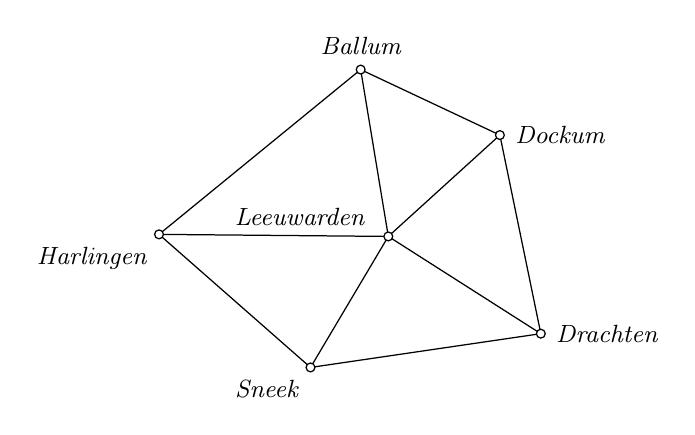
\begin{tikzpicture}[x=1.3cm,y=1.3cm,line width=.45pt,font=\small\itshape]
\coordinate (H) at (0,1.30);
\coordinate (B) at (1.97,2.91);
\coordinate (D) at (3.33,2.27);
\coordinate (R) at (3.73,.33);
\coordinate (S) at (1.48,0);
\coordinate (L) at (2.24,1.28);
\draw (H)--(B)--(D)--(R)--(S)--cycle;
\draw (L)--(H) (L)--(B) (L)--(D) (L)--(R) (L)--(S);
\foreach \p in {H,B,D,R,S,L}{\draw[fill=white] (\p) circle[radius=1.6pt];}
\node[above=2pt] at (B) {Ballum};
\node[right=2pt] at (D) {Dockum};
\node[right=2pt] at (R) {Drachten};
\node[below left=1pt] at (S) {Sneek};
\node[below left=1pt] at (H) {Harlingen};
\node[anchor=east,xshift=-.18cm,yshift=.25cm] at (L) {Leeuwarden};
\end{tikzpicture}
\end{center}
\begingroup
\makeatletter
\renewcommand{\@makefnmark}{\hbox{\normalfont[\textsuperscript{*})]}}
\renewcommand{\@makefntext}[1]{\parindent1em\noindent\hbox to1.8em{\hss[\textsuperscript{*})\ }#1]}
\makeatother
\noindent For example, the system of 6 points\footnote{Cf.\ Vol.\ IV,
pp.\ 82/87.} gives an excellent horizon closure at Leeuwarden, to within
$2^{\prime\prime}{,}197$. The angle sums in the 5 triangles are off respectively by
\[
\begin{array}{r}
1^{\prime\prime}{,}432\\
0{,}714\\
0{,}759\\
2{,}842\\
2{,}590,
\end{array}
\]
\endgroup
\makeatletter
\def\ps@gaussIXfortyone{\def\@oddhead{}\def\@evenhead{}\def\@oddfoot{\small IX.\hfil41}\let\@evenfoot\@oddfoot}
\makeatother
\thispagestyle{gaussIXfortyone}
\clearpage
\noindent322\hfill\textbf{CORRESPONDENCE.}\par\medskip
\begingroup
\makeatletter
\renewcommand{\@makefnmark}{\hbox{\normalfont\textsuperscript{*})}}
\makeatother
\noindent which are therefore also tolerable. But if one checks the
ratios of the sides, one finds that the measurements cannot be reconciled
without making much larger changes to the 10 angles on the perimeter. Under
the method of least squares they would have to be changed by
$3^{\prime\prime}{,}8$, $3^{\prime\prime}{,}6$, $3^{\prime\prime}{,}6$, $3^{\prime\prime}{,}3$, $3^{\prime\prime}{,}0$, $2^{\prime\prime}{,}7$, $2^{\prime\prime}{,}7$,
$1^{\prime\prime}{,}9$, $1^{\prime\prime}{,}1$, $0^{\prime\prime}{,}8$. If one wanted
the changes to be as small as possible, all 10 would have to be set equal,
each $=3^{\prime\prime}$\footnote{\textsc{Krayenhoff}'s own adjustment, which is not clearly set out and must be searched for, contains some much larger changes here, e.g. one of $6^{\prime\prime}{,}253$ to one angle at Drachten and one of $5^{\prime\prime}{,}530$ to an angle at Dockum, etc.}.
It is thus clear that with such measurements the sum of the 3 angles of
a triangle would often be off by more than $10^{\prime\prime}$. The figures
given are far from this, however, and so it [is] certain that at least the
values have always been \textls[120]{selected} simply to agree under
\textls[120]{this} test. In consequence, the angles must evidently often
be made worse instead of better, giving an entirely false measure of their
precision. To judge the precision of measurements properly, nothing may
be arbitrarily excluded. The easy tests using the sums of the 3 angles of
each triangle and the horizon closure are surely all too tempting, if
not to falsify, then to select and exclude, which is little better.
Unfortunately other measurements, such as those of \textsc{Delambre},
allow practically no tests beyond those mentioned. Otherwise one would
probably often find similar discrepancies.

In my system I have had the satisfaction of finding that tests of both
kinds give discrepancies of quite the same order. I am doubtful, however,
that lateral refraction could produce effects as large as the discrepancies
that appear in \textsc{Krayenhoff}'s triangles, since his sides are always so
short, his stations high in the air, and Holland is probably much less broken
up by woods than my northern terrain. The light in his system thus probably
seldom, if ever, passed as close to obstacles as it did so very often in the
latter. I would therefore be more inclined to ascribe the anomalies to
the measurements themselves.
\endgroup
